\vspace{5mm}
\section{Validazione dei sistemi implementati}
In questa sezione conclusiva vedremo i sistemi implementati in funzione, esplicandone il funzionamento durante l'esecuzione concreta degli applicativi.\newline
\subsection{Simulatore in funzione}
Partiamo dunque dal Simulatore di Piattaforma; esso, non essendo un applicativo destinato ad un uso commerciale ma bensì pensato solamente per un utilizzo aziendale in ambito di testing, non presentava dei requisiti stringenti e dispone di una GUI molto semplice e minimalista.\newline
A schermo compare dunque solo l'indispensabile al funzionamento dell'applicativo.\newline

\noindent Dipendentemente da se si dispone già o meno di un file di configurazione, nella {\bf schermata iniziale} (\emph{figura 5.3}), troviamo alcune strade che l'utente può intraprendere:
\vspace{20mm}
\begin{itemize}
    \item {\bf Creazione di una nuova configurazione}\\
    {L'utente viene portato in una pagina atta alla creazione guidata di un nuovo file di configurazione.}
    \item {\bf Modifica di una configurazione esistente}\\
    {Scegliendo questa opzione l'utente potrà caricare un file di configurazione presente nel suo dispositivo e modificarlo.}
    \item {\bf Inizio della Simulazione tramite una configurazione esistente}\\
    {Analogamente al punto precedente, viene scelto un file di configurazione e si viene portati alla schermata da dove avviare la simulazione e controllarne i parametri.}
\end{itemize}
\vspace{5mm}
\begin{figure}[H]
    \centering
    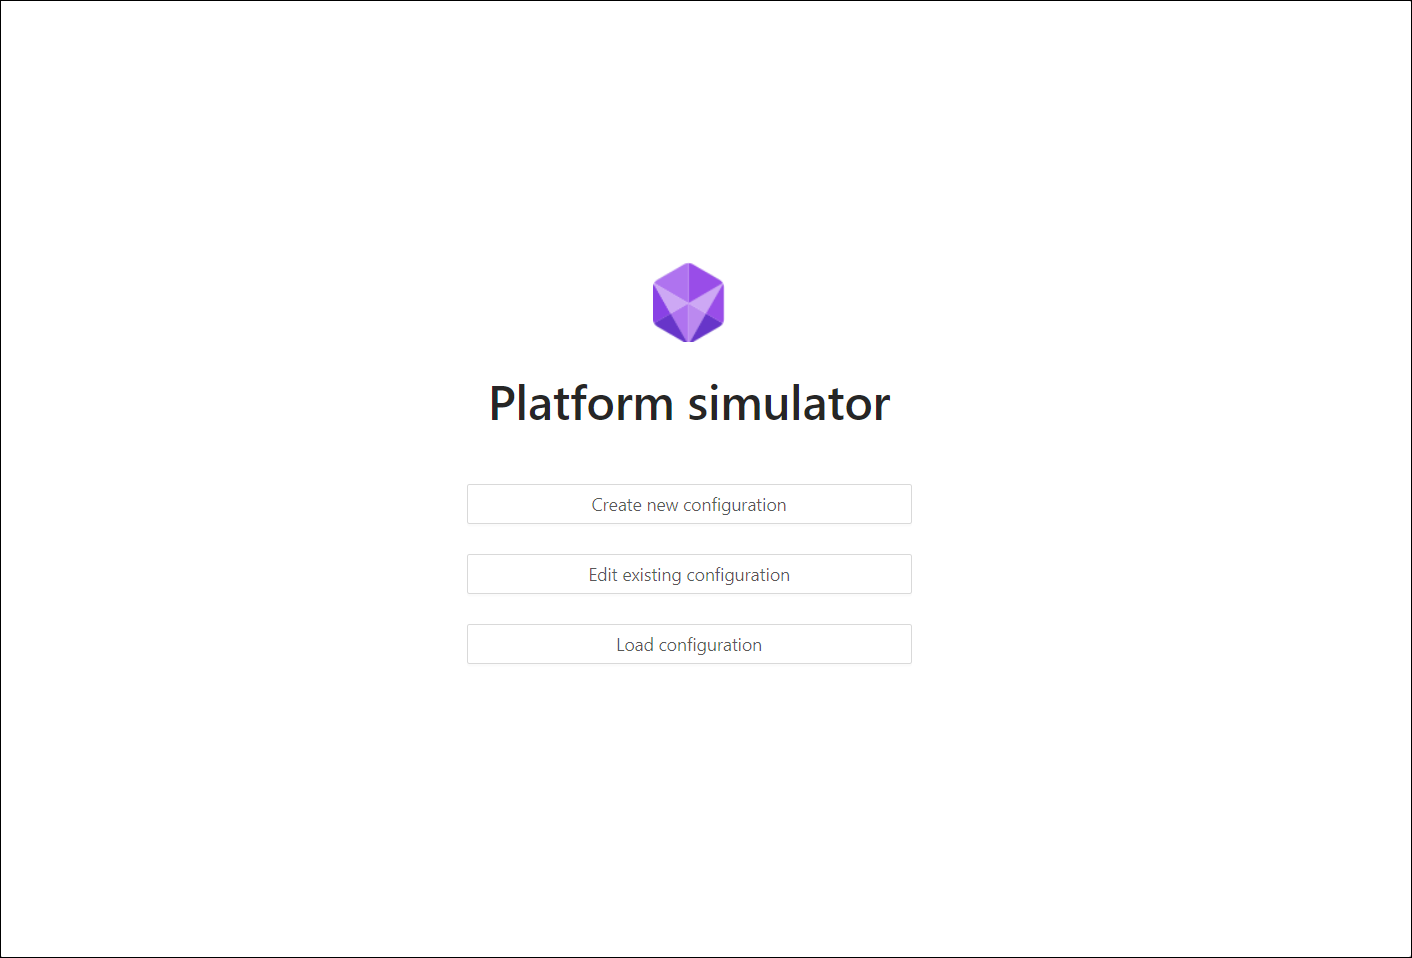
\includegraphics[width=1.0\textwidth]{img/simulator_home_screenshot.png}
    \caption{Schermata iniziale del Simulatore di Piattaforma}
\end{figure}
\vspace{5mm}
Seguendo una tra le prime due scelte dunque si viene portati alla {\bf schermata di modifica di una configurazione} (\emph{figura 5.4}).\newline

\noindent Nel caso si stia creando una nuova configurazione i campi risulteranno ovviamente vuoti mentre, nel caso si stia modificando un file, saranno caricati i valori precedentemente salvati.\newline

\noindent Partendo dalla struttura della collezione \emph{Signals} (\emph{sezione 3.3.1.1}) e con il presupposto che progetti futuri seguano quest'impostazione per salvare i dati elaborati, possiamo notare che la struttura di ogni entry sia astraibile in questo modo:
\begin{itemize}
    \item \emph{Chiave primaria composta}\\
    {I campi la cui unione rende l'entry univoca all'interno della collezione; nonostante non tutti i campi siano prevedibili a priori, sappiamo con certezza che a comporre la chiavi vi saranno i timestamp \emph{start} ed {end}.}
    \item \emph{Data}\\
    {In questo array verranno inseriti progressivamente i dati elaborati; ogni entry di questo array contiene una struttura dati.\newline
    \noindent Analogamente al caso precedente non possiamo sapere in anticipo quali siano i campi che verranno salvati ma sappiamo che in qualsivoglia struttura dati dovrà essere salvato il timestamp relativo all'istante temporale in cui quel dato è stato acquisito.}
\end{itemize}
\noindent Come conseguenza di queste considerazioni sono state definite tre macroaree di input all'interno della schermata:
\begin{itemize}
    \item {\bf Parametri MongoDB}\\
    {È qui che l'utente inserisce i dati obbligatori al fine di interfacciarsi con il database MongoDB.\newline
    \noindent Sono necessari:
    \begin{itemize}
        \item \emph{L'uri, dove reperire il DBMS}
        \item \emph{Il nome del database di riferimento all'interno del DBMS}
        \item \emph{Il nome della collezione in cui vogliamo scrivere dati}
    \end{itemize}}
    \item {\bf Chiavi}\\
    {L'utente inserisce tutte le chiavi necessarie a creare la chiave primaria composita che identifichi univocamente ogni "chunk" (entry) nella collezione (è richiesto almeno l' inserimento di una chiave).\newline
    Per ogni chiave vanno specificati nome ed valore assunto.}
    \vspace{20mm}
    \item {\bf Variabili}\\
    {Analogamente al punto precedente, in questa area vanno inserite tutte le variabili da manipolare durante la simulazione e che andranno a comporre la struttura dati di ogni entry dell'array \emph{Data}.\newline
    Per ogni variabile inserita va definito un massimo ed un minimo (oltre che il suo nome).}
\end{itemize}
\begin{figure}[H]
    \centering
    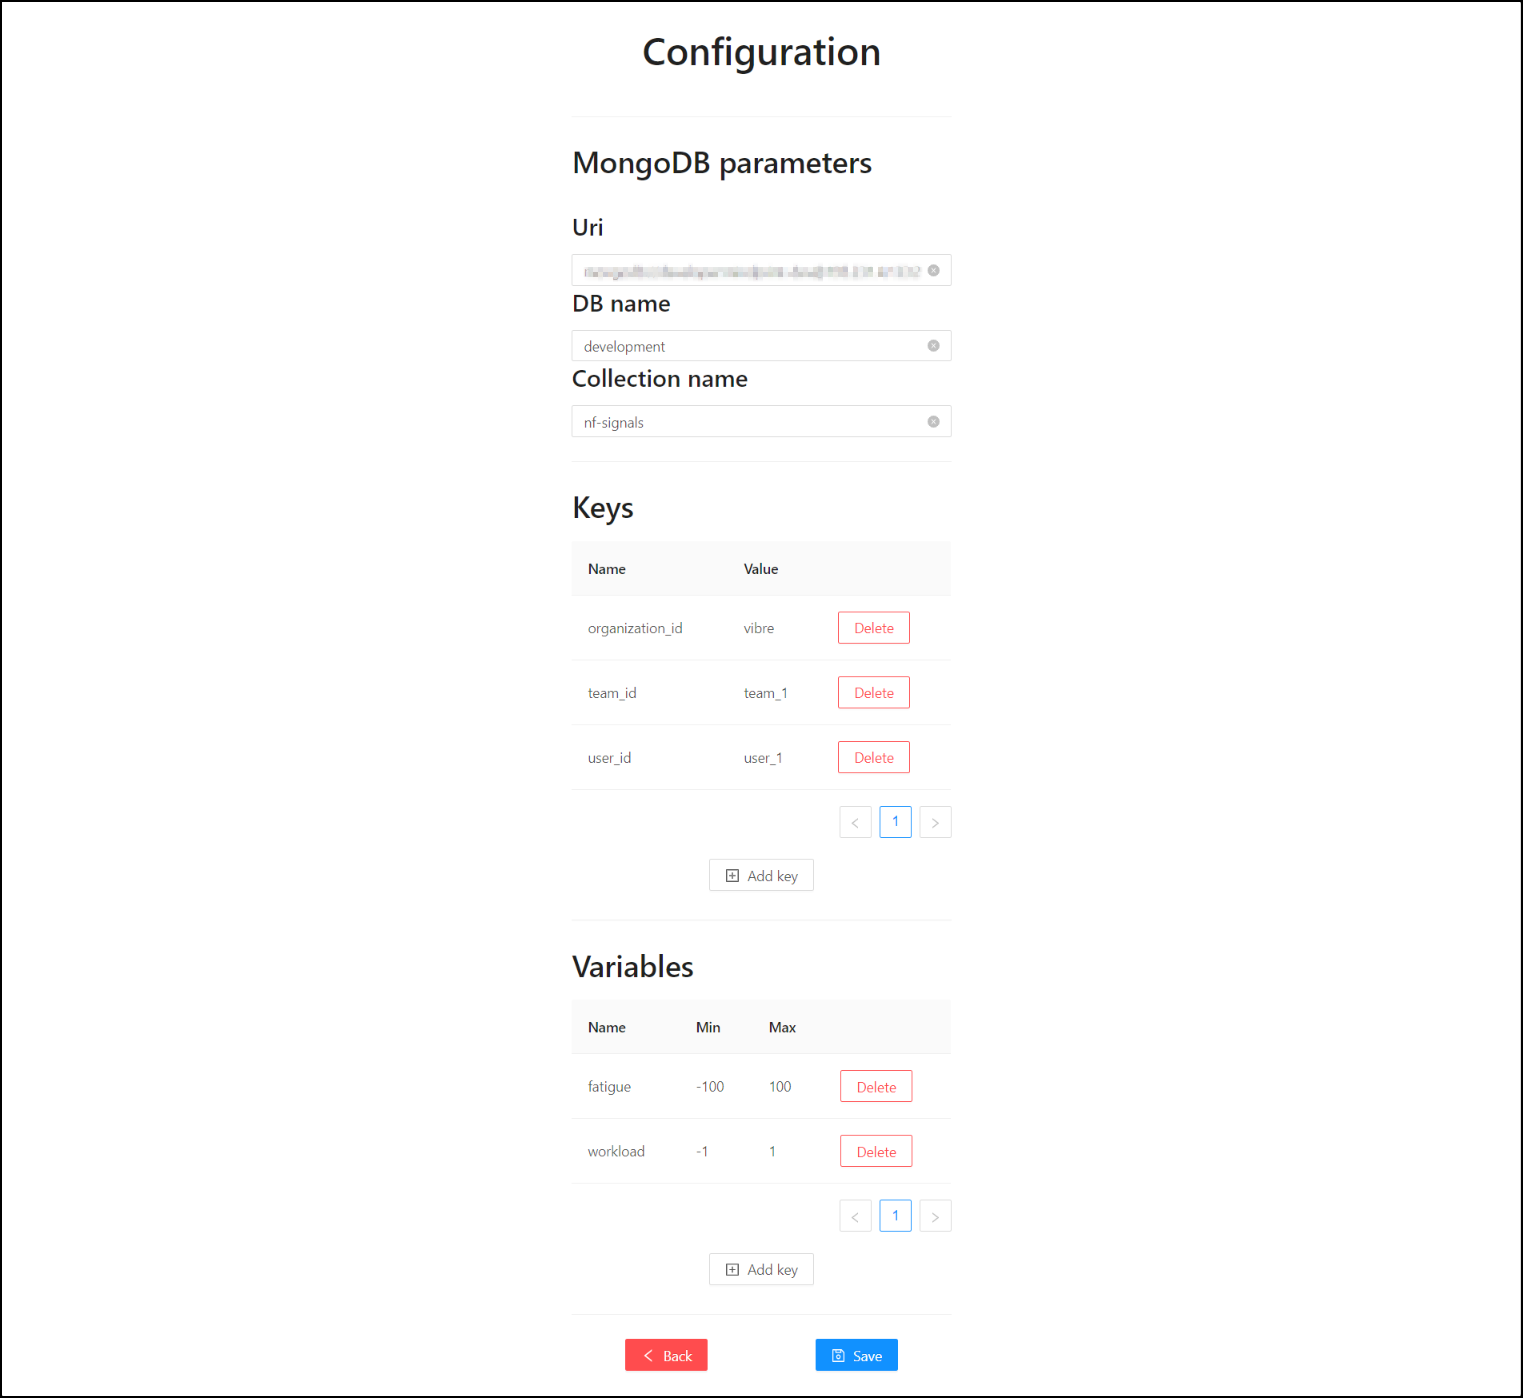
\includegraphics[width=1.0\textwidth]{img/simulator_edit_screenshot.png}
    \caption{Schermata di modifica/creazione di una configurazione con dati relativi ad una simulazione nel sistema NeuroFrame}
\end{figure}
L'ultima schermata disponibile infine è quella in cui tutte e tre le scelte iniziali possibili vanno a culminare: {\bf la schermata di simulazione} (\emph{figura 5.5}).\newline

\noindent Qui ritroviamo le tre sezioni descritte nella precedente schermata; se i parametri di connessione con il database e le chiavi non consentono interazione, nella sezione contenente le variabili ritroviamo una sottosezione per ognuno dei campi creati.\newline
È possibile modificare il valore di ogni variabile (all'interno dell'intervallo definito da \emph{max} e \emph{min}) attraverso uno slider o tramite un componente apposito che permette sia di aumentarlo/diminuirlo a piccoli step sia di specificare direttamente il valore in forma numerica.\newline

\noindent In cima alla pagina inoltre sono presenti un bottone per tornare alla schermata iniziale ed uno per iniziare/interrompere l'invio dei dati.

\noindent L'applicativo gestirà in automatico i timestamp descritti sopra in quanto campi obbligatori nella struttura di ogni chunk.
\vspace{2mm}
\begin{figure}[H]
    \centering
    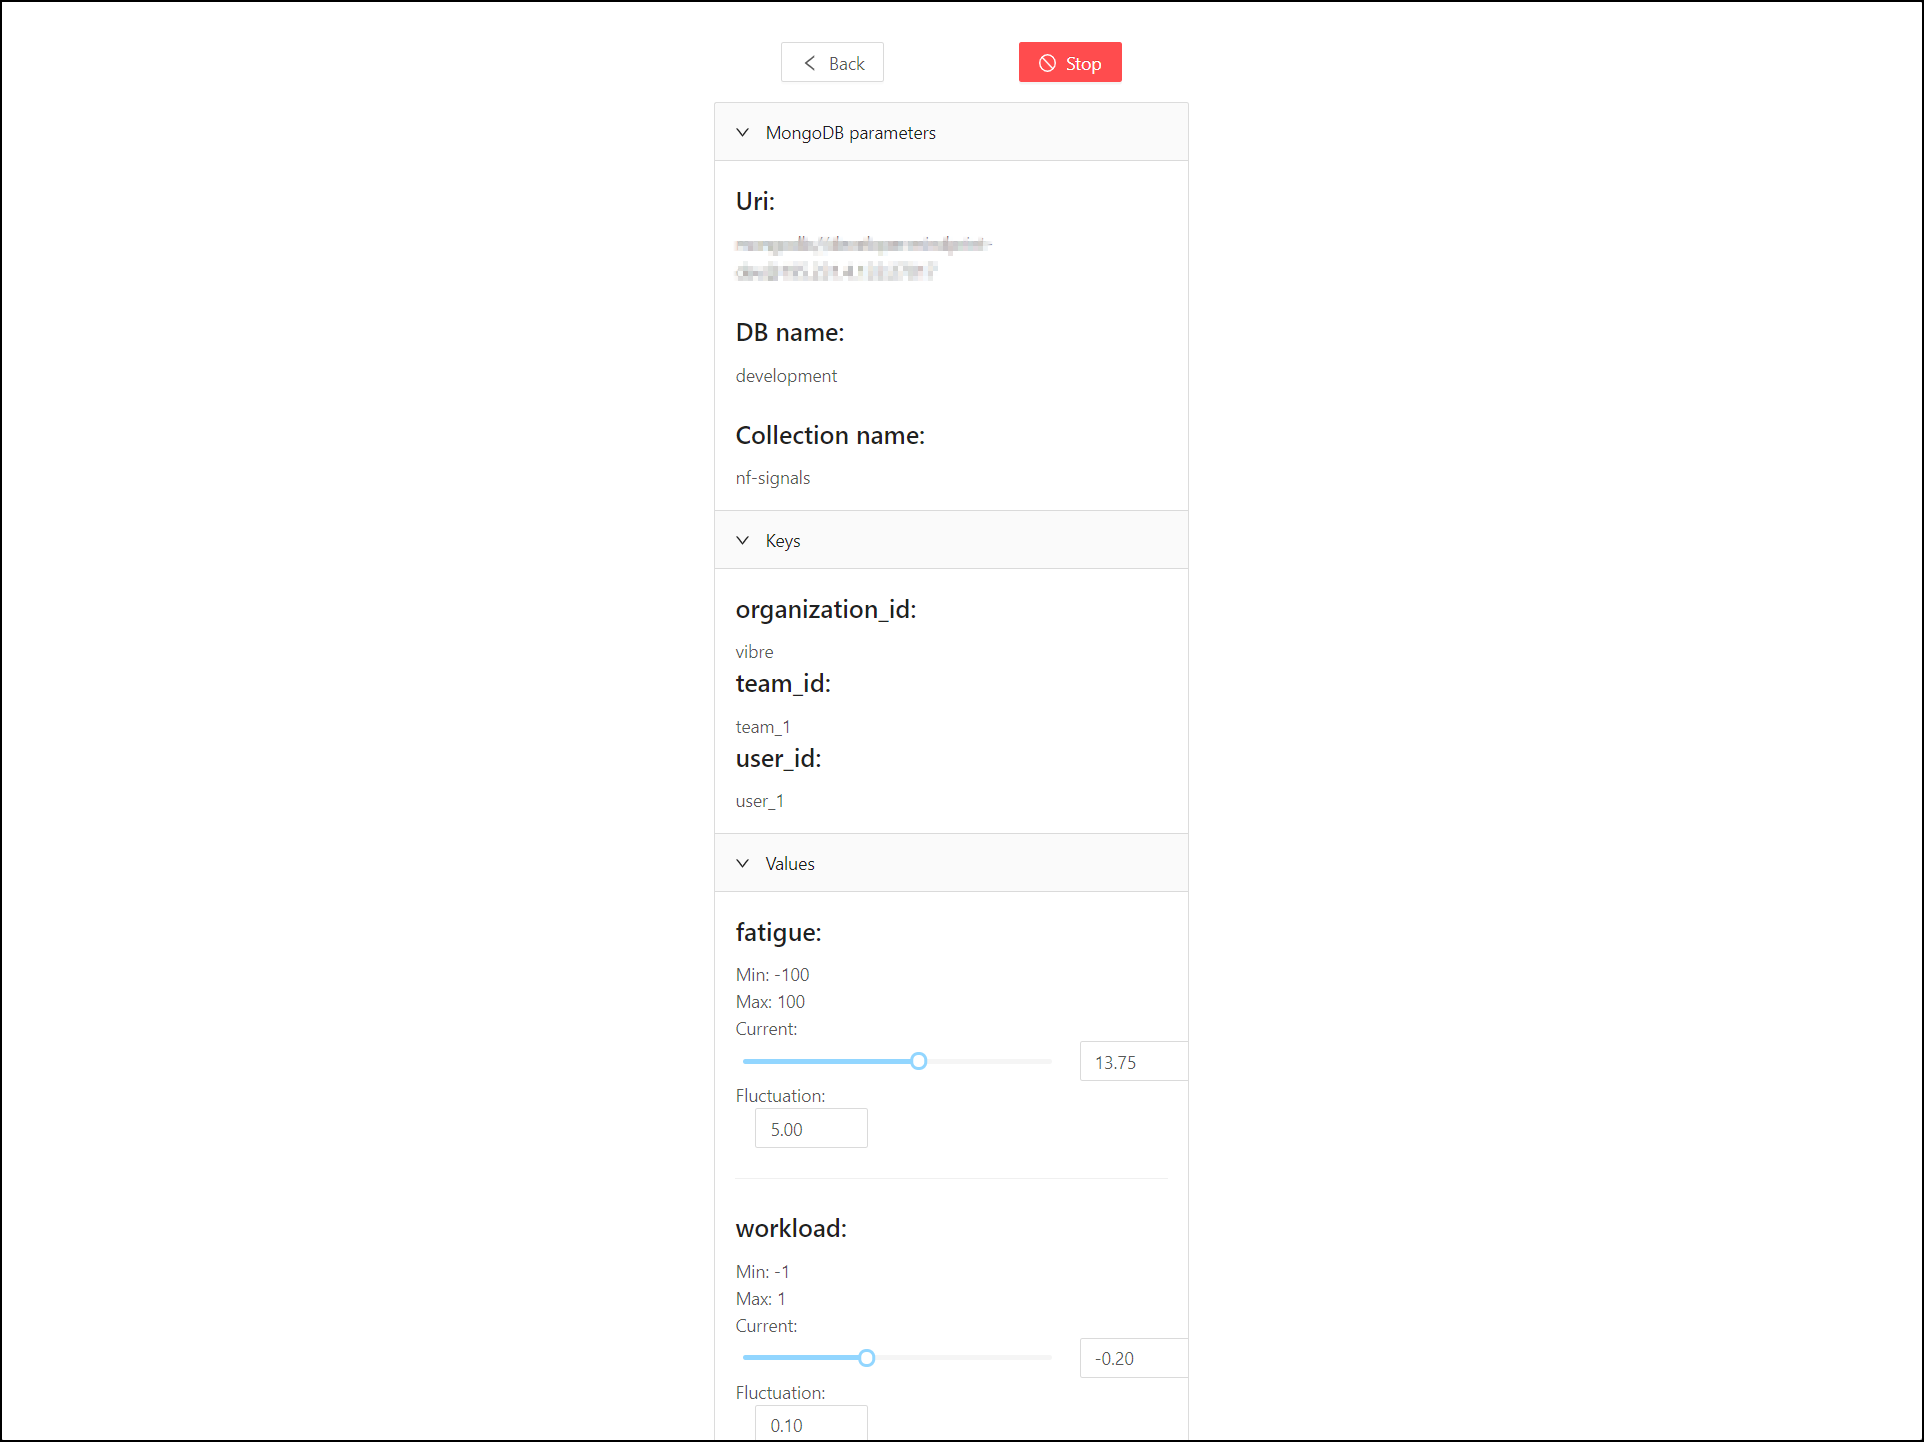
\includegraphics[width=1.0\textwidth]{img/simulator_working_screenshot.png}
    \caption{Schermata di simulazione, con invio dati correntemente in corso}
\end{figure}
\subsection{Sistema Dashboard in funzione}
Siamo finalmente giunti a visionare la Dashboard sviluppata come sottosistema di NeuroFrame.\newline

\noindent La schermata di {\bf Login} (\emph{figura 5.6}) riprende sostanzialmente in toto quanto visto nel relativo wireframe (\emph{figura 2.10}); qui troviamo un form di inserimento per le credenziali del Team manager che userà l'applicativo, nonchè il logo di Vibre.
\vspace{8mm}
\begin{figure}[H]
    \centering
    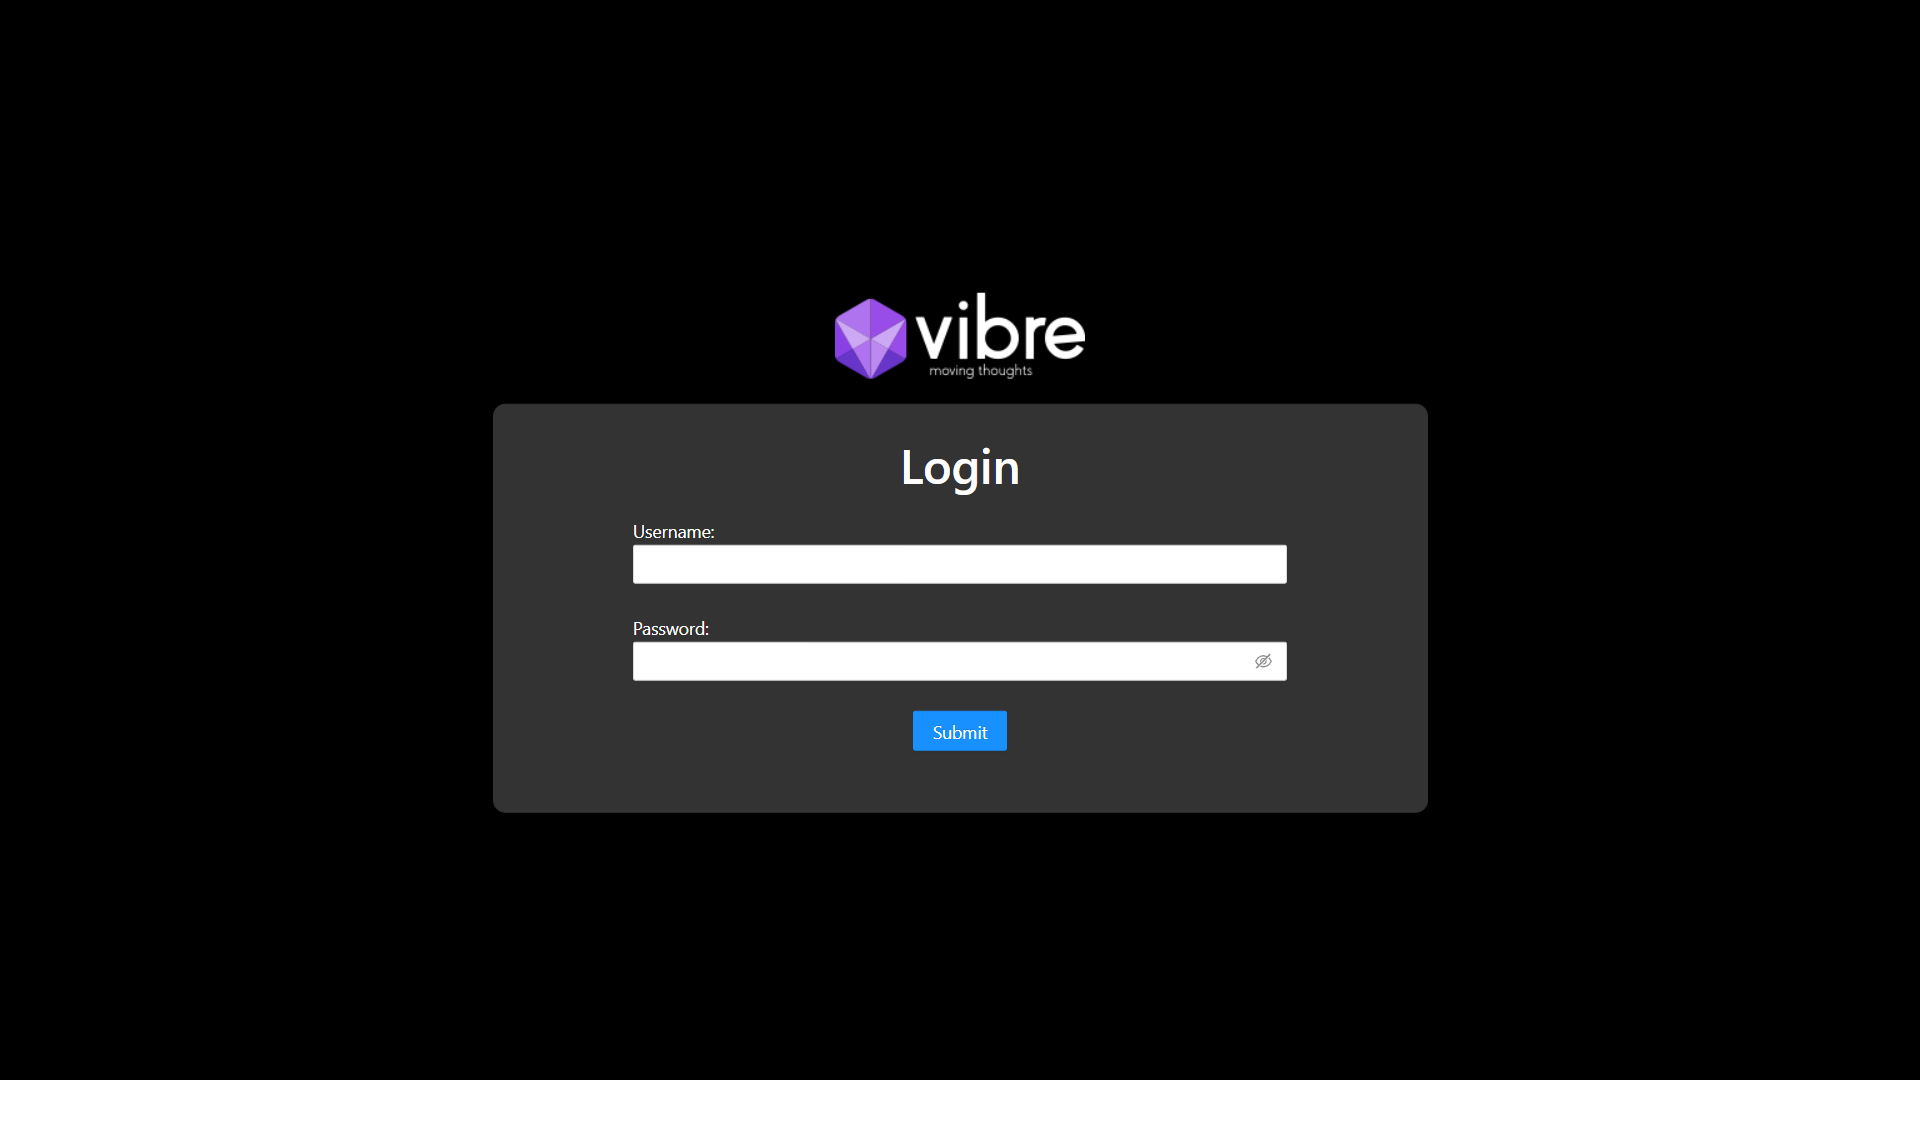
\includegraphics[width=1.0\textwidth]{img/dashboard_login_screenshot.png}
    \caption{Schermata di login del sistema Dashboard}
\end{figure}
\vspace{5mm}
\noindent Successivamente all'autenticazione del Team manager comparirà la {\bf schermata di selezione del Team} (\emph{figura 5.7}); qui saranno elencati i Team presenti all'interno dell'azienda e, per ognuno di essi, verrà mostrato l'identificativo dei suoi componenti.\newline

\vspace{30mm}

\noindent Nella barra in alto inoltre troviamo due pulsanti. Attraverso la pressione del primo pulsante si potrà accedere alla {\bf gestione dei Team} (\emph{figura 5.8}) mentre, premendo il secondo, si accederà alla {\bf gestione degli utenti} (\emph{figura 5.9}).
\vspace{8mm}
\begin{figure}[H]
    \centering
    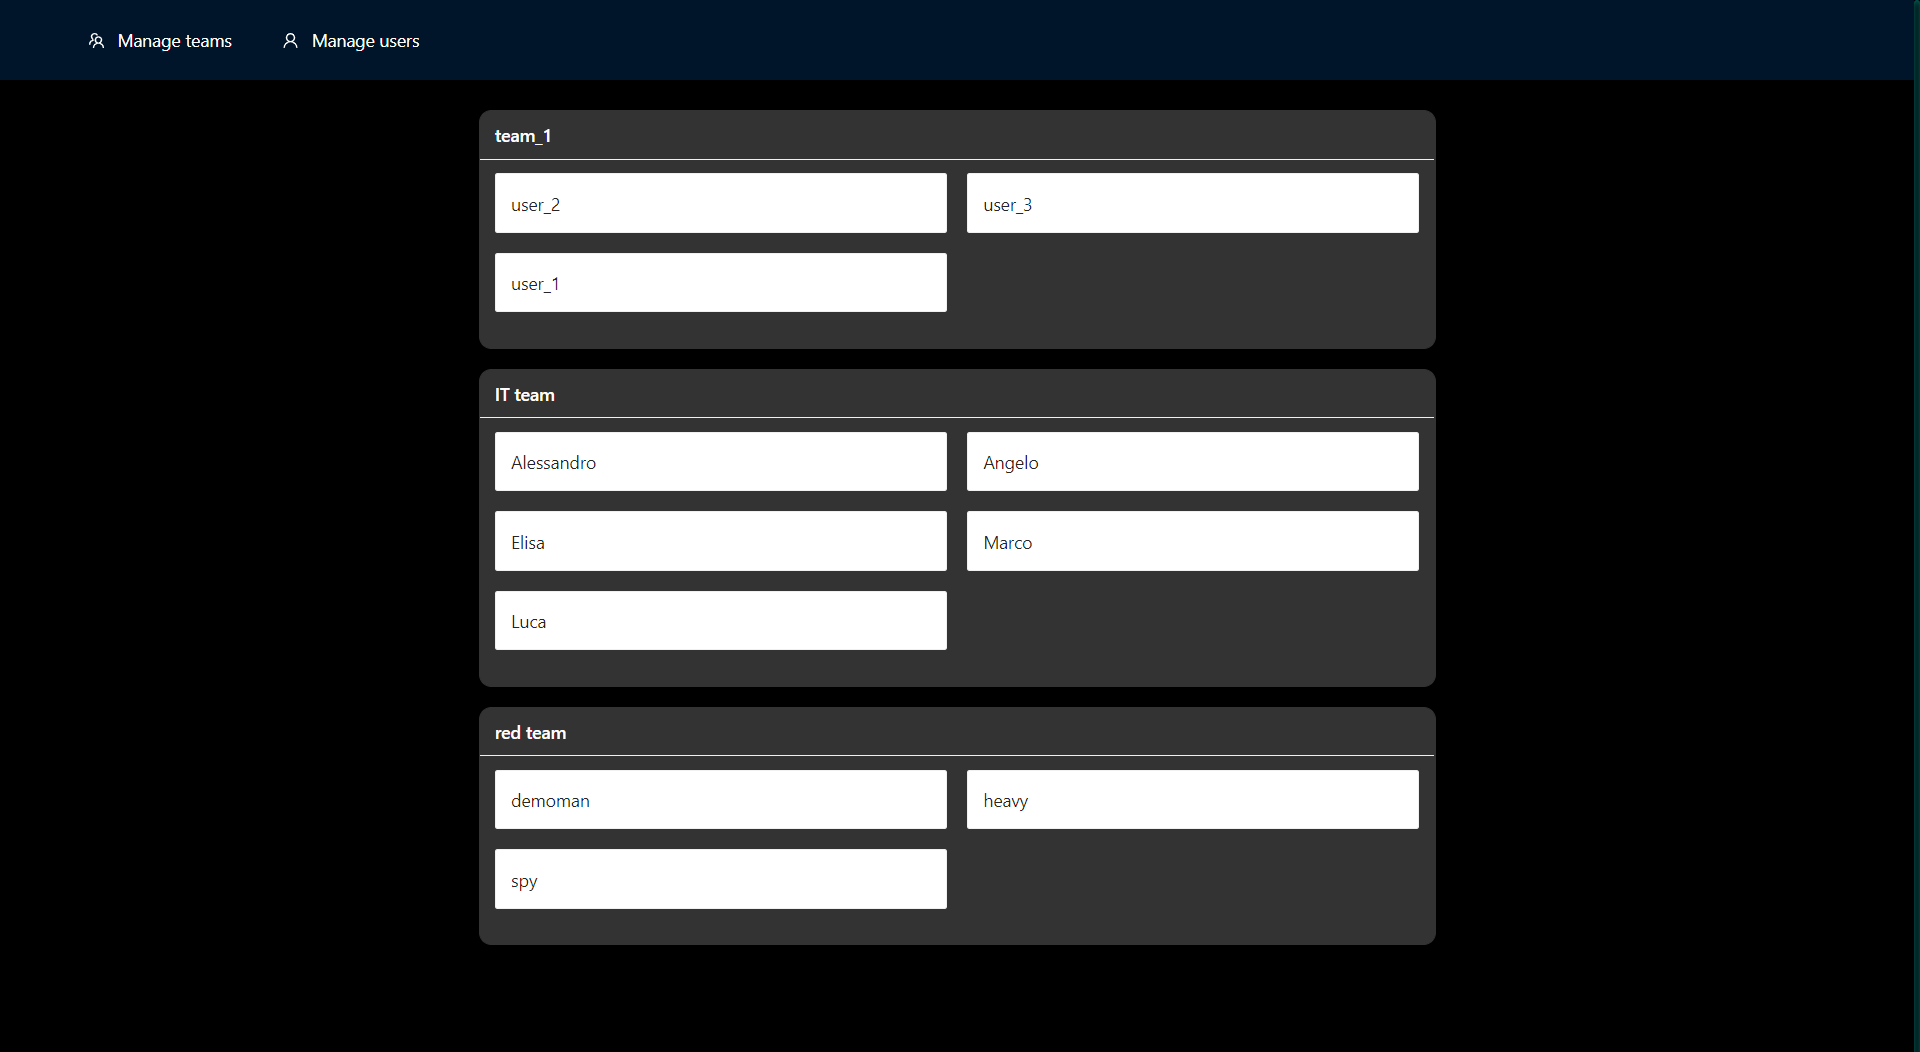
\includegraphics[width=1.0\textwidth]{img/dashboard_teams_screenshot.png}
    \caption{Schermata di selezione del Team}
\end{figure}
\vspace{5mm}
\noindent Nella schermata di gestione dei Team sarà possibile eseguire due operazioni:
\begin{itemize}
    \item \emph{Creare nuovi Team}, rispettando il numero massimo imposto dalla licenza acquistata dall'organizzazione.
    \item \emph{Eliminare Team esistenti}, previa rimozione di ogni Utente dal Team attraverso la schermata apposita che verrà affrontata successivamente.
\end{itemize}
Similmente, nella schermata dedicata alla gestione degli Utenti sarà possibile:
\begin{itemize}
    \item \emph{Creare nuovi Utenti}
    \item \emph{Eliminare Utenti che non facciano parte di un Team}
    \item \emph{Visionare un elenco degli Utenti correntemente appartenenti ad un Team; per ogni Utente verrà mostrato il relativo Team di appartenenza.}
\end{itemize}
\begin{figure}[H]
    \centering
    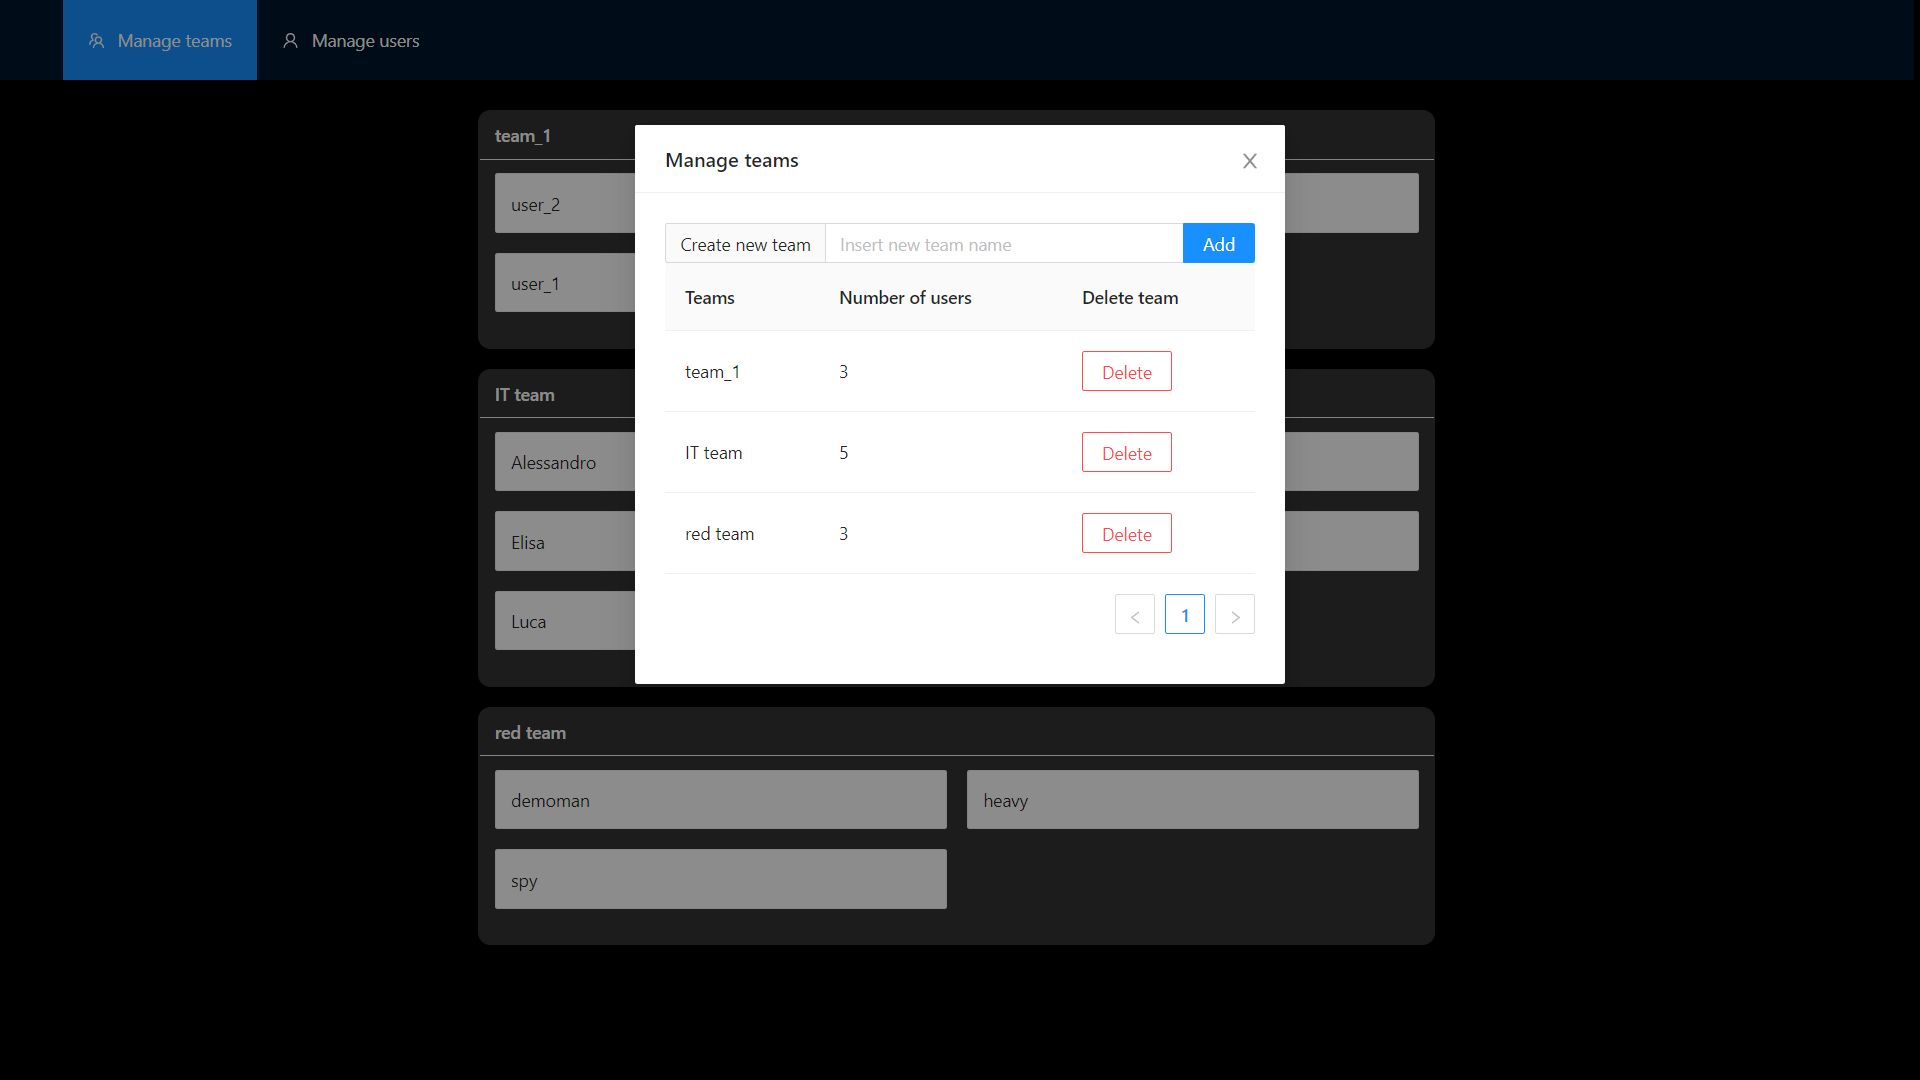
\includegraphics[width=1.0\textwidth]{img/dashboard_manage_teams_screenshot.png}
    \caption{Schermata di gestione dei Team}
\end{figure}
\begin{figure}[H]
    \centering
    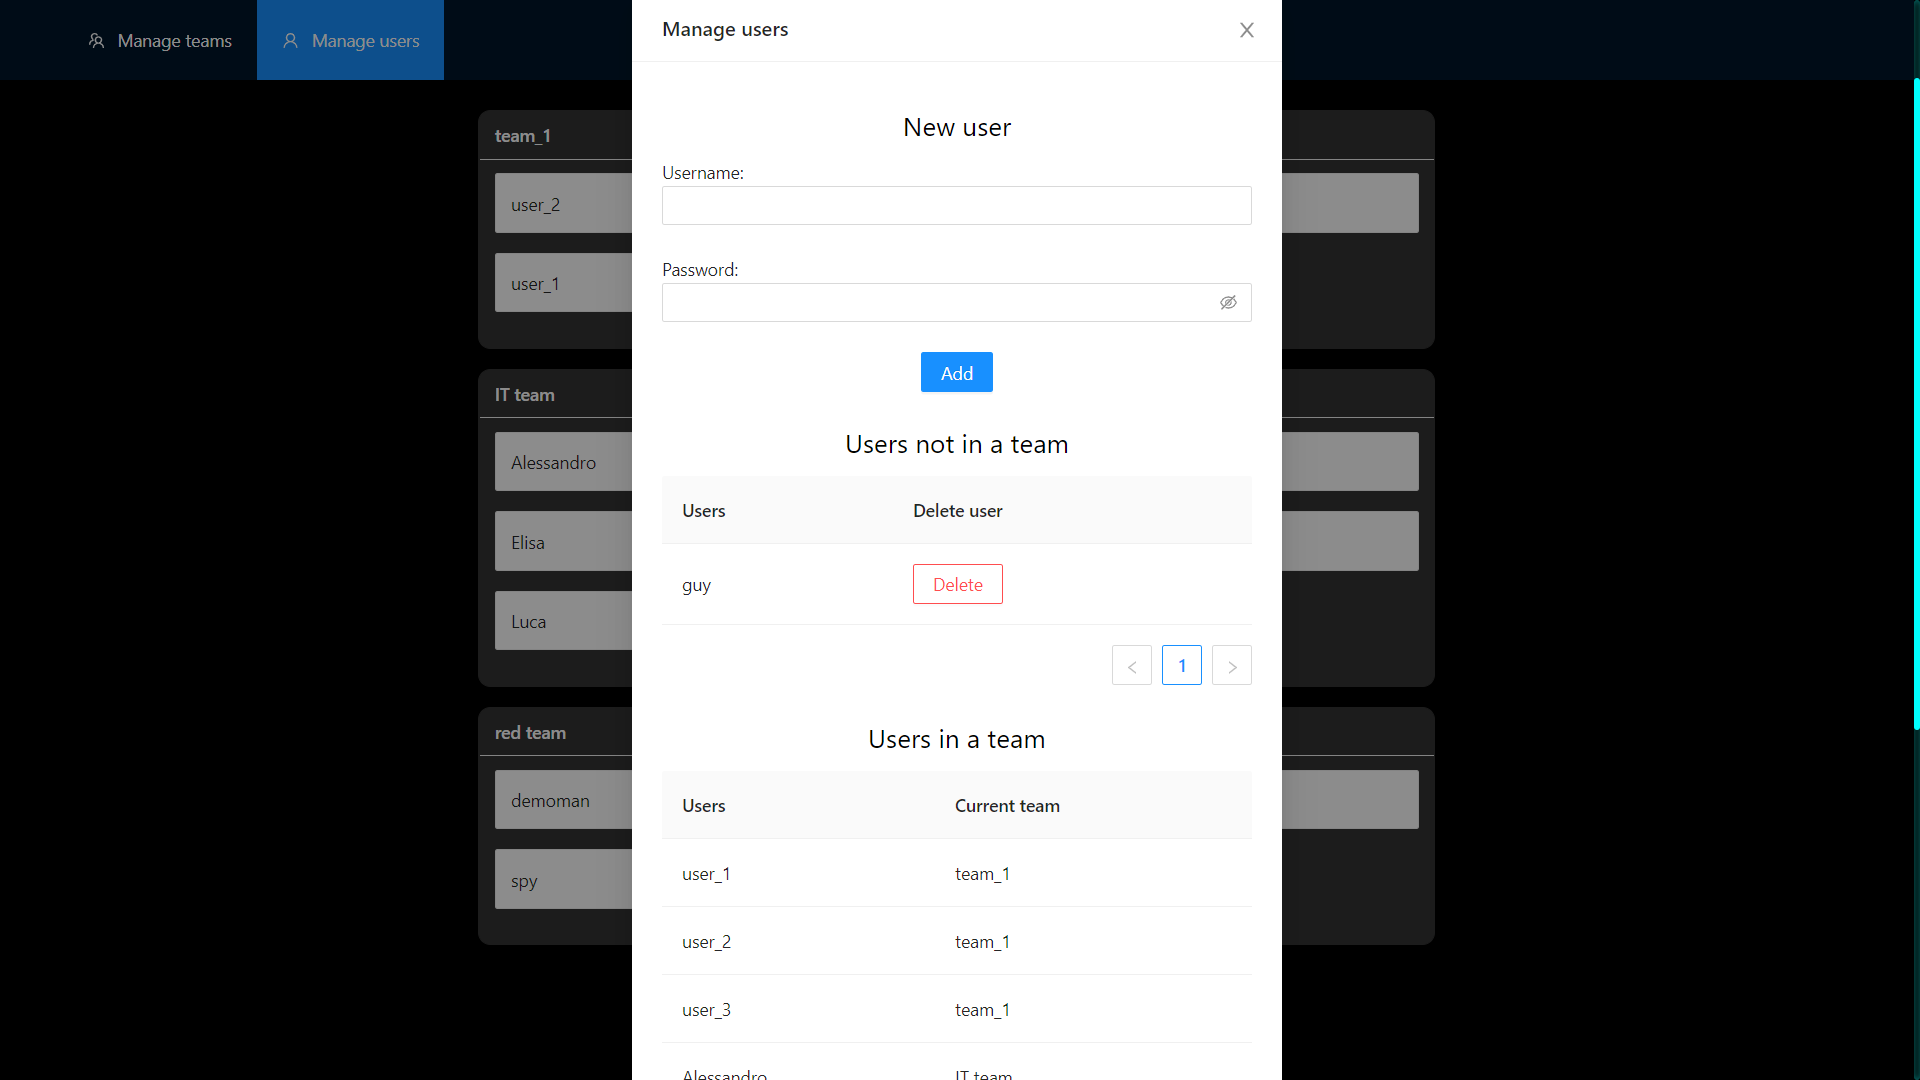
\includegraphics[width=1.0\textwidth]{img/dashboard_users_global_screenshot.png}
    \caption{Schermata di gestione degli Utenti}
\end{figure}
Una volta scelto un Team nella schermata di selezione di quest'ultimi, si viene portati nella schermata core dell'applicativo: {\bf la schermata della dashboard di monitoring del Team} (\emph{figura 5.10}).\newline
\vspace{5mm}
\begin{figure}[H]
    \centering
    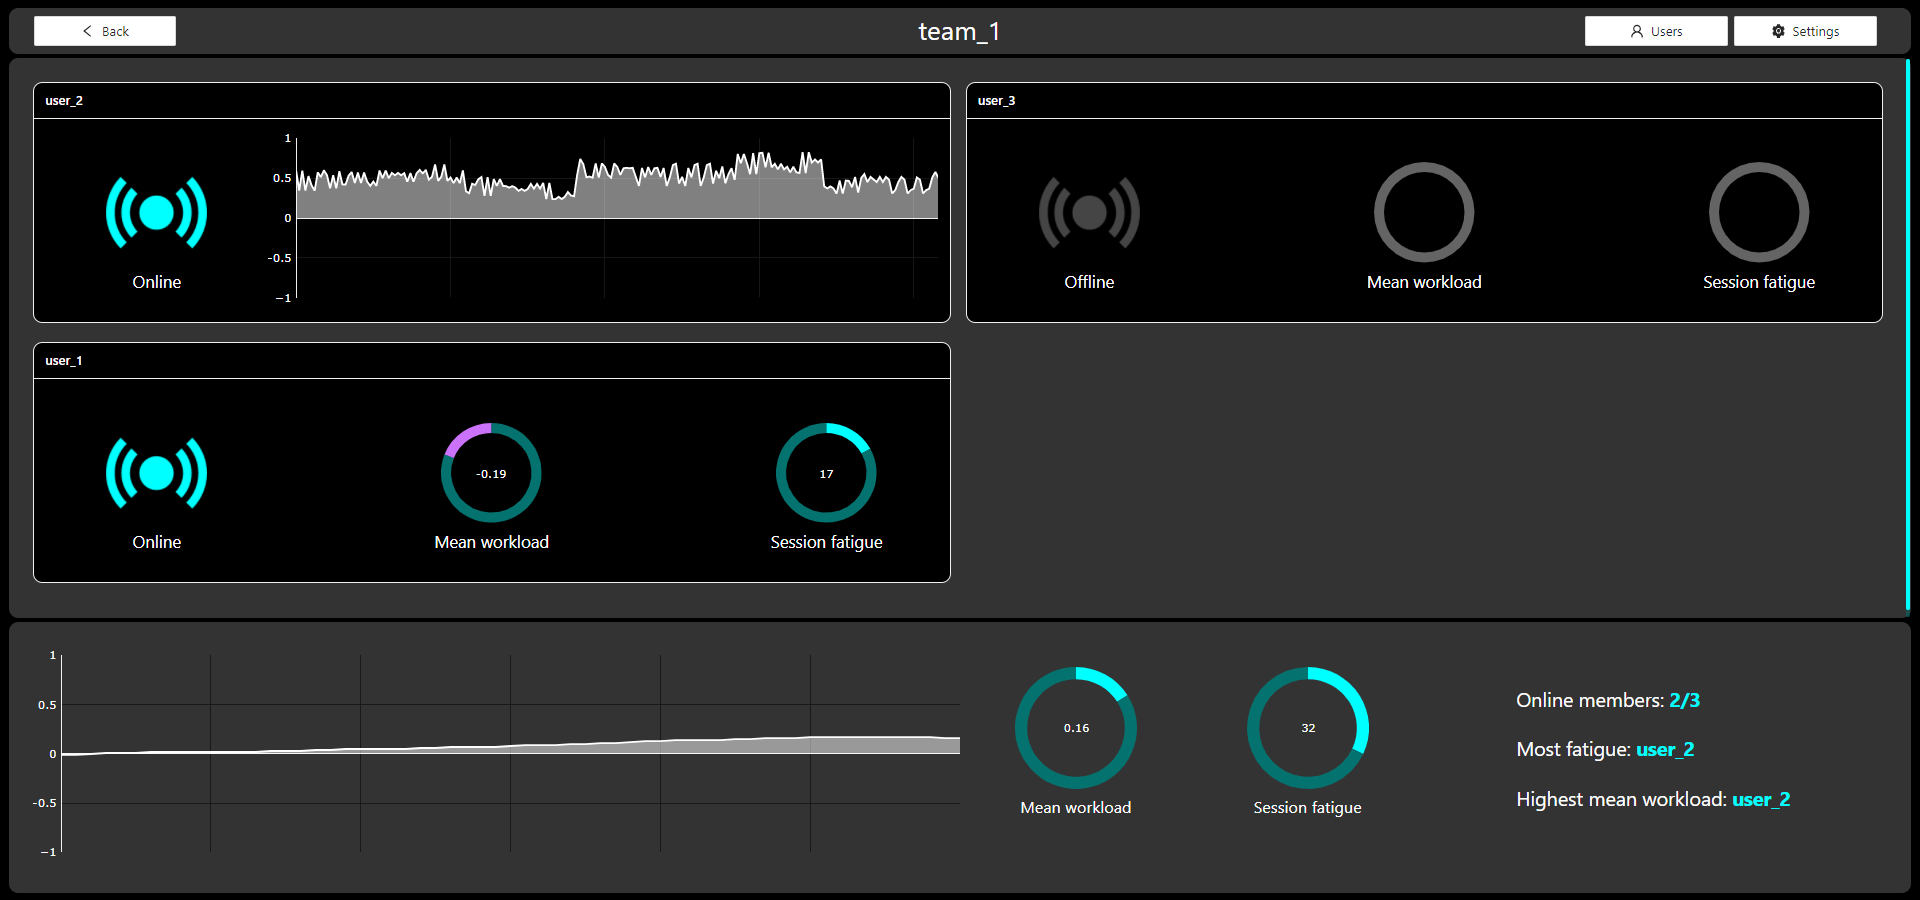
\includegraphics[width=1.0\textwidth]{img/dashboard_working_screenshot.png}
    \caption{Schermata della dashboard di monitoring del Team}
\end{figure}
\vspace{5mm}
\noindent Seguendo le linee guida del wireframe nella \emph{figura 2.11} precedentemente discussa, ritroviamo le tre macro aree pianificate:
\begin{itemize}
    \item \emph{Impostazioni}\\
    {Il risultato finale differisce leggermente da quanto rappresentato nel wireframe.\newline
    All'interno della barra delle impostazioni posizionata in cima alla pagina il logo di Vibre e quello dell'organizzazione a cui appartiene il Team leader che sta utilizzando l'applicativo sono assenti; tale assenza è da imputarsi a motivazioni legate allo spazio disponibile a schermo (ricordiamo che questa schermata deve occupare la totale altezza dello schermo senza però poter scorrere in verticale).\newline
    Sulla sinistra troviamo un bottone per tornare alla schermata di selezione del Team mentre, sulla destra, troviamo due pulsanti per le impostazioni che verranno discussi a breve:\newline
    \begin{itemize}
        \item {\bf Schermata della gestione degli Utenti del Team} (\emph{figura 5.11})
        \item {\bf Schermata delle impostazioni di visualizzazione dati} (\emph{figura 5.12})
    \end{itemize}}
    \item \emph{Area singoli componenti}\\
    {In quest'area è presente una sezione dedicata ad ogni componente del Team.\newline
    Essendo il numero di Utenti non prevedibile a priori questa è l'unica sezione della schermata che può scorrere in verticale.\newline
    Per ogni Utente suddividiamo gli indicatori in due aree:\newline
    \begin{itemize}
        \item \emph{Indicatore di connessione}\\
        {Descrive lo stato di connessione dell'Utente in questione.\newline
        Al momento può assumere solo uno stato booleano (online o offline) ma, in versioni future, è prevista la possibilità di visualizzare la qualità del segnale inviato dall'Utente durante lo streaming dati.}
        \item \emph{Indicatori delle metriche neurali}\\
        {Qui vengono mostrate le metriche calcolate dall'algoritmo MindPulse (o fornite dal Simulatore).\newline
        
        \noindent In figura vediamo, per lo \emph{user 1}, la visualizzazione di \emph{carico cognitivo medio} e \emph{affativamento medio} tramite grafici a torta; data la possibilità di queste metriche di assumere anche valori negativi, i grafici si riempiono in senso orario (con colore azzurro) all'aumentare in valori superiori allo zero mentre, per valori negativi, si riempiono in senso antiorario (con un colore viola chiaro).\newline
        Valori positivi simboleggiano rispettivamente un utilizzo di risorse mentali (per il carico cognitivo) ed un affaticamento mentale dell'individuo; di contro quando queste metriche assumono valori negativi l'utente sarà meno concentrato e più rilassato.\newline
        Superati dei valori critici, i grafici assumono una colorazione rossa ed il sistema avvisa il Team manager che, ad esempio, consiglierà all'Utente stanco una pausa.\newline
        
        \noindent Per lo \emph{user 2} troviamo invece una diversa rappresentazione dei dati; l'affaticamento non viene mostrato ed inoltre, attraverso un grafico cartesiano, non viene mostrata la media del carico cognitivo bensì \emph{i valori che esso assume nel tempo}(è su questi valori difatti che la media viene calcolata).
        
        \noindent Per cambiare la modalità di visualizzazione delle metriche neurali sarà sufficiente un click del Team manager nello spazio dell'Utente d'interesse.}
    \end{itemize}
    }
    \item \emph{Area del Team}\\
    {Qui vengono mostrate a schermo delle metriche che riassumono la condizione generale del Team.\newline
    A sinistra troviamo un grafico cartesiano che descrive l'andamento \emph{della media} di tutti i carichi cognitivi nel tempo.\newline
    Subito a destra ritroviamo i grafici a torta prima affrontati, rappresentanti le medie attuali rispettivamente di carico cognitivo e di affaticamento mentale.\newline
    Infine è presente una sezione con delle info quali numero di Utenti online, quale sia l'Utente più affaticato al momento così come l'utente con carico cognitivo maggiore.}
\end{itemize}

\noindent Riprendendo il discorso che concerne le schermate riguardanti le impostazioni, analizziamo in primo luogo quella riguardante la gestione degli Utenti del Team (\emph{figura 5.11}).\newline
Il Team manager in questa schermata può rimuovere Utenti dal Team o aggiungerne di nuovi che non siano già appartenenti ad un Team.\newline
Il sistema impedirà di aggiungere Utenti nel caso si sia raggiunto il numero massimo di Utenti per Team consentito dalla licenza acquistata dall'organizzazione.
\vspace{5mm}
\begin{figure}[H]
    \centering
    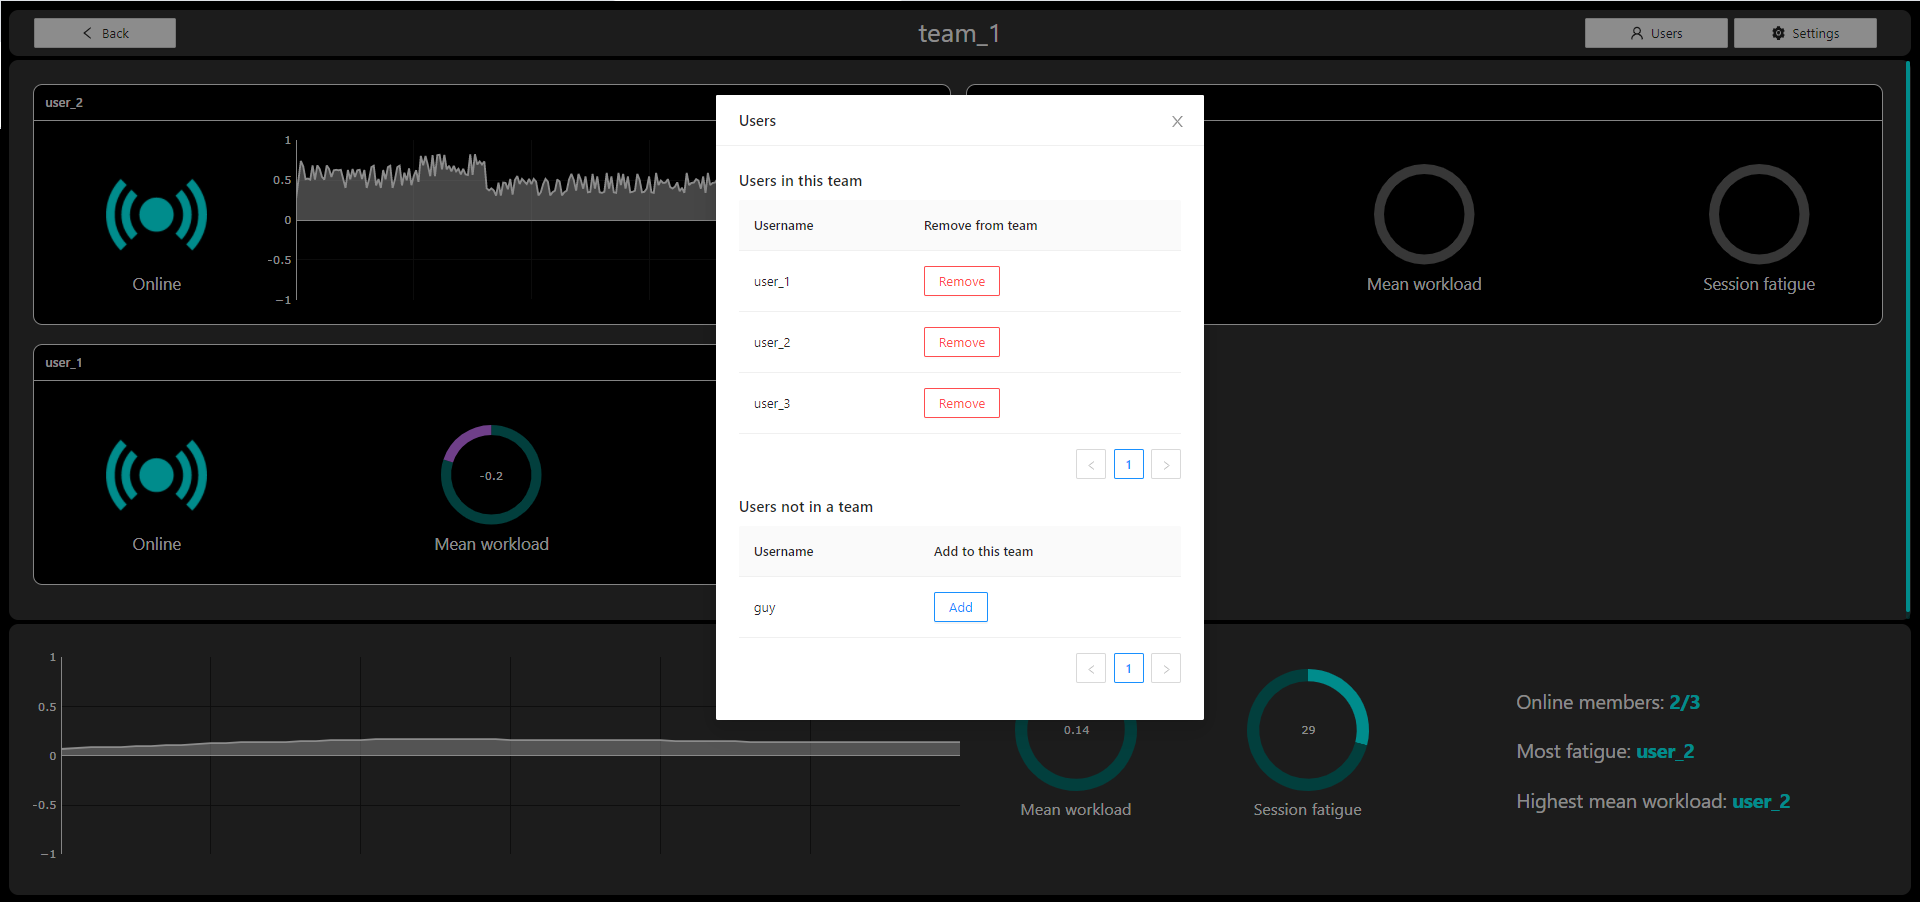
\includegraphics[width=1.0\textwidth]{img/dashboard_team_users_screenshot.png}
    \caption{Schermata della gestione degli Utenti del Team}
\end{figure}
\vspace{5mm}
\noindent La seconda schermata di opzioni invece riguarda le impostazioni di visualizzazione dati(\emph{figura 5.12}).\newline
I cambiamenti in questa sezione saranno relativi solamente alla modalità di visualizzazione dati del Team manager che sta utilizzando l'applicativo e non si ripercuote su altri Team manager della stessa organizzazione.\newline

\vspace{20mm}
In questa prima versione sarà possibile agire su due parametri:
\begin{itemize}
    \item \emph{Modificare la finestra temporale per il carico cognitivo}\\
    {Attraverso questo parametro verrà impostato lo span temporale rappresentato dai grafici cartesiani rappresentanti l'evoluzione temporale del carico cognitivo nel tempo.\newline
    Ad esempio, impostando 60 secondi, i valori più vecchi di tale parametro non verrebbero più visualizzati nei grafici cartesiani e, conseguentemente, non verrebbero nemmeno considerati per il calcolo del carico cognitivo medio.\newline
    È stato imposto un limite superiore di 300 secondi per evitare un possibile rallentamento del sistema dato dalle risorse limitate del browser.}
    \item \emph{Modificare il valore massimo assoluto dell'affaticamento mentale}\\
    {Se la metrica restituita da MindPulse riguardo il carico cognitivo è inclusa in un range che va da -1 a 1, l'affaticamento mentale invece non dispone né di un limite inferiore né di un limite inferiore.\newline
    Studi e test al riguardo hanno verificato che in situazioni ordinarie tale valore non cresca oltre una certa soglia, fissata di default a -100 e 100 nella Dashboard.\newline
    Un limite superiore ed inferiore è necessario al funzionamento sopra descritto dei grafici a torta; nel caso compaiano valori che superino i limiti, essi verranno comunque mostrati in forma numerica al centro del grafico che, però, non si riempirà oltre la capienza massima, sia positiva che negativa.\newline
    Viene però fornita la possibilità di variare il valore assoluto di tale range nel caso durante l'utilizzo compaiano frequentemente valori fuori anomali fuori scala.}
\end{itemize}
\vspace{2mm}
\begin{figure}[H]
    \centering
    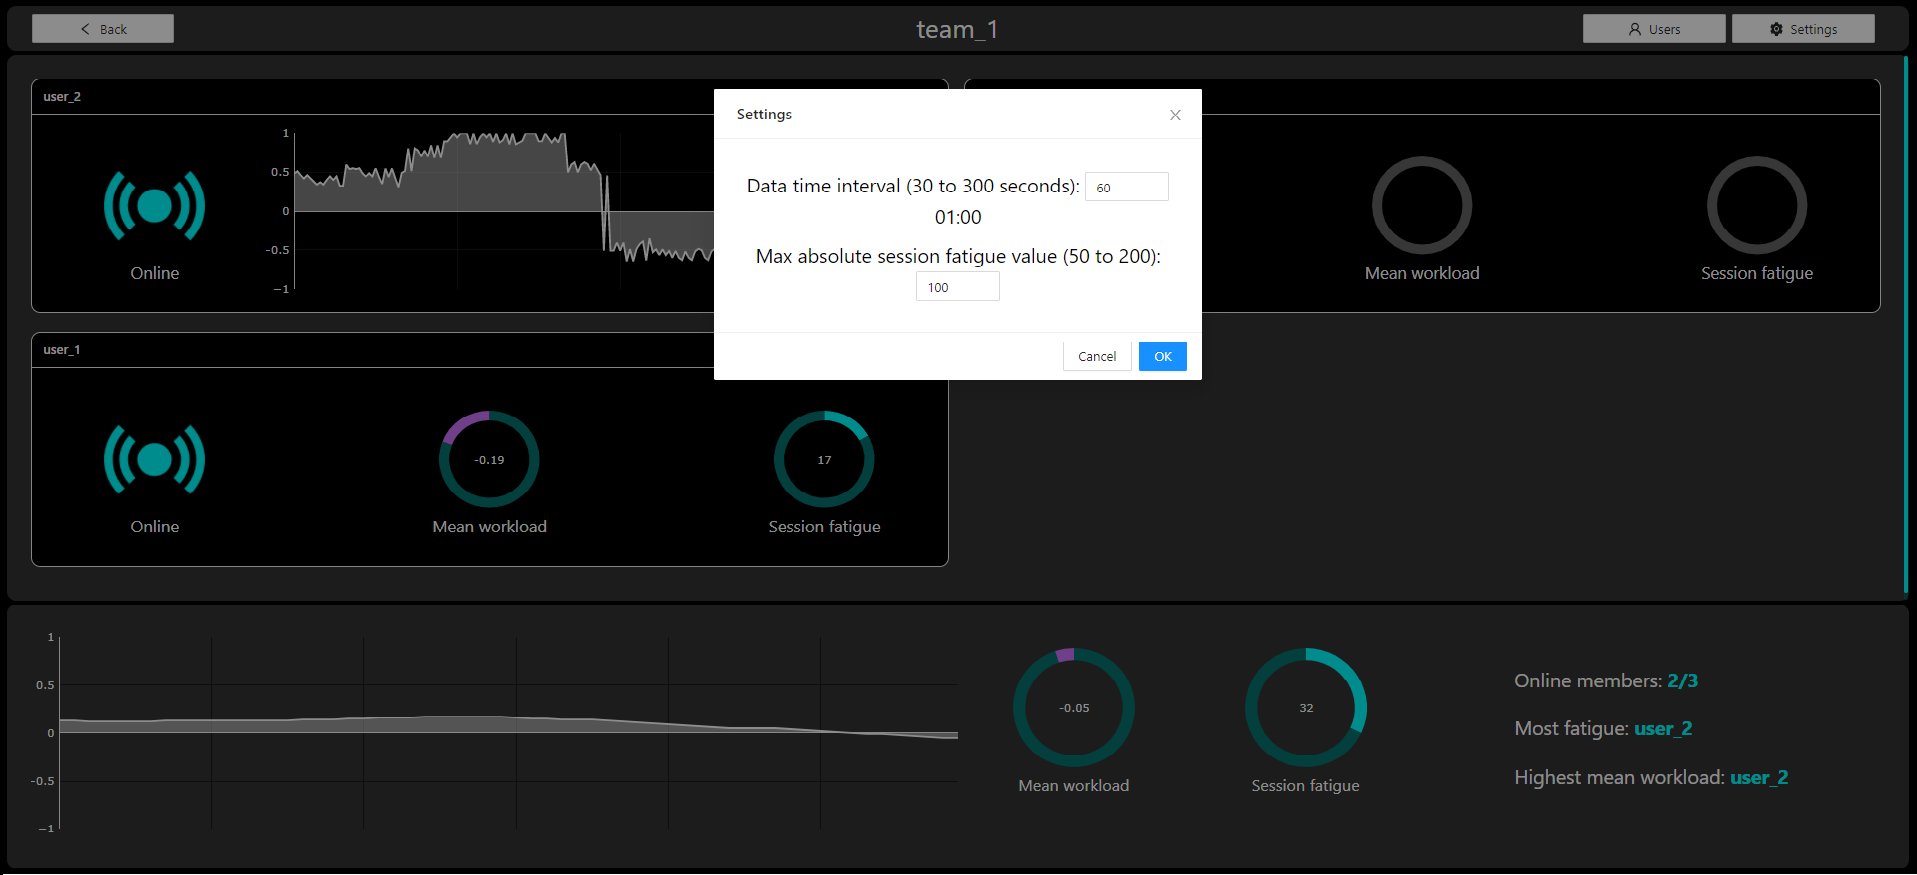
\includegraphics[width=1.0\textwidth]{img/dashboard_team_settings_screenshot.png}
    \caption{Schermata delle impostazioni di visualizzazione dati}
\end{figure}